\chapter{Object-relational Mapping}

Die folgenden Strategien haben sich für einen \ORM bewährt und lassen sich auch größtenteils in der Literatur wiederfinden. Höchstwahrscheinlich existieren in der Praxis noch viel mehr implementierte Lösungen für diese Problematik. Dadurch, dass viele Hersteller eine eigene, unabhängige \ORM-Lösungen entwickeln mussten, weil es lange Zeit keine benutzbare, öffentliche Library oder Ähnliches gab, gibt es eine Vielzahl von unterschiedlichen Ansätzen. Es ist schwer sich für einen richtigen Lösungsansatz zu entscheiden, da sich von Fall zu Fall die Anforderungen stark unterscheiden. Die möglichen Schwerpunkte durch die sich die Lösungen unterscheiden sowie Vor- und Nachteile sollen in späteren Kapiteln weiter untersucht werden. Deshalb werden hier zunächst die meist genutzen, in der Literatur am meisten genannten und in der Praxis etabliertesten Strategien vorgestellt.

\section{Speichern des Zustandes eines Objektes}

Die Konvention, die in den meisten \term{Mappings} getroffen wurde ist, dass eine Klasse als eine Relation (Tabelle) im Datenbankschema dargestellt wird. Der Name der Relation ist der Name der Klasse. Die Attribute (Spalten) der Relation sind die Attribute der Instanz der Klasse. \\
Den Zustand eines Objektes kann man also persistent speichern, indem man die Ausprägungen aller Attribute des Objektes in die Relation einfügt. Ein Mapping (welches auch sehr simpel sein kann) wandelt dabei den Typen des Ob\-jekt\-attri\-but\-es in den Typen der Tabellenspalte um. Eine Instanz eines Objektes wird dann durch ein Tupel in der Klassenrelation repräsentiert. \\
Dadurch, dass ein Tupel in einer Relation eindeutig unterscheidbar sein muss, kann es sein, dass weitere Eigenschaften zur Klasse hinzugefügt werden müssen. Diese nennt man auch \term{Shadow information}. Die \term{Shadow Information} ist häufig ein künstlicher numerischer Schlüssel, der sich für jedes neu eingefügte Tupel der Relation automatisch um 1 erhöht. Somit ist gewährleistet, dass jede Instanz der Klasse -- auch wenn ihre Attribute gleich sind -- eindeutig unterscheidbar ist. Dieses Prinzip wird Eindeutigkeit der Objektidentität genannt. Ich schreibe OID für \term{Object Identifier} und meine damit jene \term{Shadow information} die ein Objekt in der Applikation und in der Datenbank eindeutig identifiziert. Meist haben Objektinstanzen in objektorientierten Programmiersprachen eine eigene eindeutige Identität. Diese ist nicht als \term{Shadow information} verwendbar, da beim Laden eines Objektes aus der Datenbank eine neue Instanz der Klasse mit den Werten aus der Datenbank befüllt wird. Dabei besitzt dann das eben geladene Objekt A in der Applikation eine andere Identität als ein weiteres Objekt B, welches das selbe Tupel in der Datenbank repräsentieren kann. Dies ist in fast allen \term{Mappern} unerwünscht, da man nun nicht mehr Änderungen in Objekt A auf Änderungen in Objekt B beziehen kann und man unerweigerlich Konflikte beim Speichern von Objekt A und Objekt B erhält. Ich gehe also -- wenn nicht anders genannt -- davon aus, dass in der Applikation zu jedem Zeitpunkt für jedes Tupel einer Klassenrelation nur eine Objektinstanz existiert.

\section{Speichern von Klassenhierarchien}

Die Modellierung einer Klassenhierarchie im relationalen Schema ist eines der komplexen Probleme des \IM. Trotzdem wurde mit der Zeit mehr als nur eine Variante gefunden. Es gibt mehrere \term{Mappings} für die Darstellung der Vererbung:\\

\subsection{Horizontales Mapping}
Jede Klasse der Hierarchie besitzt eine eigene Tabelle. In jeder Tabelle werden alle Attribute der eigenen Klasse A und die Attribute der Klassen, von denen Klasse A geerbt hat, als Spalten eingetragen. Die Attribute der Elternklassen werden also auf jede Kindklasse dupliziert.\\
Die Beziehung zwischen der Relation der Kindklasse und der Relation der Elternklasse wird meistens gar nicht abgebildet. Das heißt die Information, dass Klasse A Kind von Klasse B ist, ist nur im objektorientierten Model bekannt. Das Mapping ist also mit dieser Darstellung der Vererbung nicht bidirektional (Es gibt keine Möglichkeit ein ausschließlich relationales Model in ein objektorientiertes Model zu transformieren, wenn dieses Mapping benutzt wird). Um eine Klasse aus der Hierarchie zu laden, muss genau eine Tabelle abgefragt werden. Jedoch gibt es Probleme, wenn die Struktur einer Klasse weit unten in der Hierarchie geändert wird. Wird z.~B. ein Attribut umbenannt, muss die Änderung in allen Kindklassen ebenfalls erfolgen. Dieses Ändern ist fehleranfällig und aufwendig.

\subsection{Vertikales Mapping}
\begin{anmerkung}[Tiefe einer Klassenhierarchie]Ich bezeichne die Tiefe der Klassenhierarchie als die Anzahl der Eltern und rekursiv dessen Eltern von einer Klasse. Wird also Klasse A von Klasse B abgeleitet und Klasse C von Klasse B dann ist die Tiefe der Hierarchie von A,B und C = 3.
\end{anmerkung}
\noindent Jede Klasse der Hierarchie besitzt eine eigene Tabelle, jedoch werden die Attribute der Elternklassen nicht in den Kindklassen dupliziert. Jede Relation der Kindklasse besitzt einen Fremdschlüssel auf den Schlüssel der Relation der Elternklasse (mehrere bei Mehrfachvererbung). Ein Objekt der Kindklasse K abgeleitet von Elternklasse E kann also nur aus der Datenbank geladen werden, wenn das Tupel aus der Relation K und das dazu passende Tupel der Relation E geladen wird. Die Eltern Klasse kann jedoch wiederum von einer weiteren Klasse abgeleitet sein.\\
Je nachdem wie tief die Klassenhierarchie ist, ist der gespeicherte Zustand eines Objektes auf mehr als eine Tabelle verteilt. Für eine sehr tiefe Klassenhierarchie müssen also für das Laden eines Objektes sehr viele Tabellen abgefragt werden. Das Ändern der Struktur einer Elternklasse ist kein Problem, da es keine Duplikate der Attribute gibt. Jede Klasse kapselt seine Attribute in seiner Relation.\\

\subsection{Filter-Mapping}
Um die komplette Hierarchie abzubilden wird nur eine Tabelle benutzt. Alle Instanzen der Klasse werden als Tupel in dieser Tabelle repräsentiert. Alle Attribute der kompletten Hierarchie befinden sich nur in dieser Tabelle. Da beim Einfügen eines Tupels von Klasse A nicht alle Spalten von Klasse B benötigt werden, muss es erlaubt sein dass ein Tupel der Klassentabelle leere Attribute der Klasse B bzw. A besitzt. Da dadurch ein Tupel eingefügt werden kann, dessen Attribute alle leer sind (außer der OID), muss die Zugehörigkeit eines Tupels zu der Klasse in der Hierarchie als \term{Shadow information} gespeichert werden. Meist geschieht dies durch eine weitere Spalte der Tabelle mit dem Namen der Klasse zu der das Tupel gehört. Diese Spalte wird deshalb auch Filter (bei Hibernate \term{Discriminator}) genannt und gibt der Strategie den Namen. Dadurch dass jedes Feld (bei disjunkten Klassenattributen) leer sein darf, ist es nicht mehr möglich durch das relationale Schema die Integrität der Daten zu gewährleisten. Auch ist es möglich Attribute in der Datenbank zu speichern, die nicht zur Klasse des Tupels gehören. Die Applikation muss alle Abfragen mit dem Kriterium für den Filter erweitern, somit muss oft ein Index über den \term{Discriminator} gelegt werden, damit diese Abfragen performant bleiben.\\

\subsection{Generelles Mapping}
\begin{anmerkung}[Namen von Relationen]
\tabelle{Namen von Relationen} (Tabellen) eines Schemas werde ich \tabelle{rekursiv} markieren.
\end{anmerkung}
\noindent Beim generellen \term{Mapping} erhält keine Klasse der Hierarchie eine eigene Relation. Die komplette Struktur einer Klasse (Name der Klasse, alle Attribute, der Name der Elternklasse(n)) wird in einem generellen Schema dargestellt. Eine Relation dieses Schemas speichert z.~B. die Namen der Klassen und die Referenz auf eine Elternklasse. Eine andere Relation modelliert die Namen und Typen der Attribute und die Zugehörigkeit zu einer Klasse.\\
\begin{figure}[htbp]
  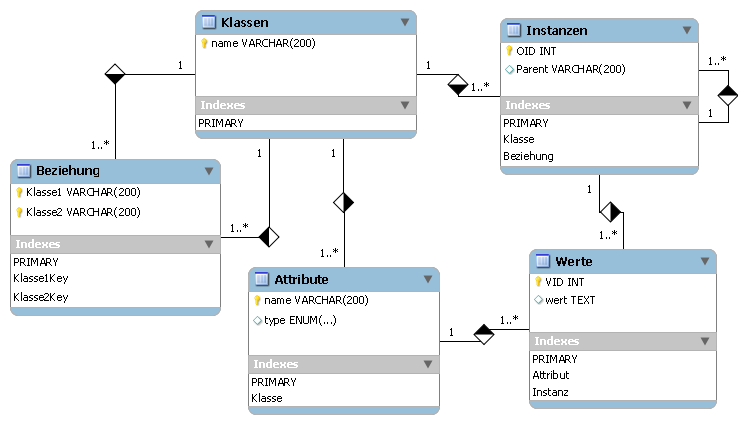
\includegraphics[width=\textwidth]{figures/generic_mapping_structure}
  \caption{Beispiel einer Struktur für generelles Mapping}
  \label{generic_mapping_structure}
\end{figure}
\noindent Die Abbildung \ref{generic_mapping_structure} zeigt ein Beispiel für ein solches Schema. In \tabelle{Klassen} sind die Namen aller Klassen der objektorientierten Applikation gelistet. In \tabelle{Beziehungen} sind Vererbungen, Assoziationen und Kompositionen von Klassen gespeichert. Jede Klasse besitzt n Attribute, deshalb gibt es eine Beziehung zu \tabelle{Attribute}, die wiederum Objekte mit Werten verbindet. In \tabelle{Werte} stehen alle Werte aller Objekte in der Applikation. Jede Instanz in der Tabelle \tabelle{Instanzen} hat eine eigene OID (\term{Shadow Information}). Eine Instanz kann von einer anderen Instanz abgeleitet sein, oder mit einer anderen Instanz eine Beziehung haben (z.~B. Vererbung).

\section{Speichern von Beziehungen zwischen Objekten} \label{orm-beziehungen}

Die Beziehungen zwischen Objekten können so wie Beziehungen zwischen Relationen im klassischen relationalen Datenbankschema gelöst werden. Je nach Multiplizität der Beziehung (1:1 1:n oder n:m) werden Fremdschlüssel der Relation B in der Relation A angelegt, wenn A und B eine Beziehung eingehen. Bei einer Multiplizität von n:m muss eine weitere Beziehungsrelation eingefügt werden, die von Relation A und Relation B jeweils einen Fremdschlüssel speichert (Zwischentabelle). \\
Dieser klassische Ansatz reicht für die meisten Applikationen aus und der Großteil der \ORM-Software benutzt diesen auch. Dennoch wird z.~B. in \cite{lodhi-ghazali} noch eine andere Möglichkeit beschrieben: Für jede Beziehung zwischen Objekten wird eine Beziehungsrelation eingefügt (Zwischentabelle wie bei n:m im klassischen Fall). Je nach Multiplizität werden in der Tabelle beide Fremdschlüssel einzeln (1:1), nur eine Seite (1:n) oder beide kombiniert mit Unique-Constraints belegt. Der Grund für die zusätzlichen Tabellen im Schema ist, dass z.~B. bei einer Beziehung zwischen Relation A und Relation B mit Multiplizität 1:n der Fremdschlüssel beim klassischen Schema in Relation B eingefügt werden muss. Betrachtet man die Beziehung aus der Sicht von Relation A, ist nicht mehr zu erkennen, dass eine Beziehung zu Relation B überhaupt besteht. Es ist auch nur Relation B für die Pflege der Beziehung verantwortlich. Dies entspricht nicht dem Prinzip der Kapselung von Informationen im Objekt der Relation A. Außerdem kann die Liste der Fremdschlüssel in einer Relation, die an besonders vielen Beziehungen beteiligt ist, schnell sehr lang werden. Durch eine empirische Untersuchung kommt \cite{lodhi-ghazali} zu dem Schluss, dass die Lösung mit vielen Beziehungsrelationen ungefähr gleich schnell im Vergleich zu der klassischen ist.

\section{Laden und Marshalling von Objekten} \label{marshalling}

Das Laden von Objekten wird in den meisten \ORM-Lösungen zu unausführlich behandelt. Mit einer naiven Idee lässt sich das Problem meist zufriedenstellend lösen. Es ist z.~B. sehr einfach ein einzelnes Objekt mit einer gegebenen Objekt-ID aus der Datenbank zu laden und die passende Instanz in der objektorientierten Applikation zu erstellen:
\begin{itemize}
\item Die Datenbank muss nach dem Tupel für die Objekt-ID angefragt werden.
\item Die Werte des Tupels müssen in die Attribute des Objektes überführt werden (\term{Marshallling}).
\end{itemize}
Kritisch wird es jedoch, wenn man eine größere Menge von Objekten gleichzeitig laden will. Der naive Ansatz -- der zwar das Prinzip der Kapselung von Eigenschaften und Methoden einhält -- scheitert hier an der Leistungsfähigkeit. Für eine Menge von \mth{n} Objekten werden \mth{n} simple Abfragen an die Datenbank getätigt, anstatt eine große Abfrage zu tätigen und über das Ergebnis zu iterieren. Hier kommt die Eigenart des \IM besonders gut hervor: Jedes Objekt möchte seine eigenen Abfragen an die Datenbank verwalten (Kapselung), aber bei relationalen Abfragen werden Objekte in großen Mengen zurückgegeben (Performanz).\\
Ein weiterer wichtiger Aspekt ist die Entscheidung wie die Anfragen an das System gestellt werden. Am häufigsten werden diese drei Möglichkeiten benutzt:
\begin{enumerate}
\item Alle Abfragen werden in reinem SQL geschrieben. Der Entwickler muss dafür Sorge tragen, dass alle Informationen für jedes Objekt vollständig vorhanden sind. (reines SQL).
\item Die Abfragen werden in einem Abfrageobjekt mit einer objektorientierten API gekapselt. Diese Struktur wird später in reines SQL umgewandelt (objektorientierte SQL API).
\item Es wird eine eigene Abfragesprache definiert, die große Ähnlichkeiten mit SQL hat. Die Sprache vereinfacht den Umgang mit Objekten und wird ebenfalls später zu reinem SQL transformiert. (eigene Abfragesprache).
\end{enumerate}
Es stellt sich die Frage, ob es besser ist dem Anwender eine bekannte Anfragesprache als API zur Verfügung zu stellen (wie z.~B. SQL) oder aber alle Details für das Laden von Objekten in abstrakten Methoden der objektorientierten Applikation zu kapseln (2.). Die Meinungen, ob die Anfragesprache als SQL oder als abstrakte Query Sprache umgesetzt werden sollte, gehen weit auseinander. Somit wird in \cite[S. 7]{ambler-persistence-layer} die Benutzung von SQL als Verletzung gegen das Prinzip der Kapselung angesehen. Wenn in der Applikation SQL direkt benutzt wird, bindet man die Applikation dauerhaft an das Datenbankschema. Man verliert dadurch die Möglichkeit das Design des Schemas dem \term{Mapper} zu überlassen. Ebenso wird die Schnittstelle zur Datenbank nicht mehr abstrahiert, d.~h. die Applikation ist von einem bestimmten \DBMS abhängig. Wird das \DBMS gewechselt, muss auch die Applikation aufwendig geändert werden. Das Design der Abfragesprache wird als besonders schwierig betrachtet. Die Sprache soll in der Domain des Objekt-Models konstruiert werden, aber muss mächtig genug sein, um alle komplexen SQL-Abfragen, die sonst geschrieben werden würden, behandeln zu können (\cite[S. 24]{russel-bridging}). Die Entscheidung SQL, eine objektorientierte SQL API oder eine eigene Abfragesprache zu entwerfen, ist deshalb sehr komplex und viele Lösungen kann man an diesem Merkmal unterscheiden.\\

\section{Vertiefung: Object Loading}\label{object-loading}

Bevor ich im nächsten Kapitel auf verschiedene konkrete Implementierungen eingehen werde, möchte ich zunächst ein Thema noch weiter vertiefen:\\
Das Laden von Objekten scheint nicht oft Inhalt von wissenschaftlichen Arbeiten zu sein, obwohl dort meiner Meinung nach die besten Optimierungen bezüglich Performanz möglich sind. \\
Beginnt man eine \ORM-Lösung naiv zu implementieren könnte man schnell zu folgender Struktur kommen:\\
\begin{itemize}
\item Jede Klasse, die persistent gemacht werden soll leitet eine Basisklasse ab, in der die Persistenzmechanismen als Methoden zur Verfüung stehen (\code{save(), get(), delete()})
\item Es gibt eine Methode \code{get()} mit dem Parameter OID, welche den verknüpften Datensatz aus der Datenbank lädt (Verbindung herstellen, SQL absetzen, Daten auslesen, \code{init()} aufrufen)
\item Es gibt eine weitere Methode \code{init()}, die die Werte aus dem Ergebnis der Abfrage von \code{get()} in die Attribute des Objektes überführt. Die Methode \code{init()} ordnet also den Attributen eine Zeile des Abfrageergebnisses zu.
\end{itemize}
Diese Lösung scheint erst einmal sehr simpel und funktional zu sein. Die Klassen, die persistent gemacht werden sollen (Entity-Klassen), müssen die Basisklasse nur ableiten und \code{init()} so überschreiben, dass die speziellen Attribute der Klasse mit Daten gefüllt werden, sobald \code{get()} aufgerufen wird.\\
\\
Ich stelle nun ein programmiertes Beispiel vor, bei dem ein Teil des Bei\-spiel-""Daten\-bank\-schemas (Anhang \ref{beispiel-datenbankschema}) benutzt wird. In diesem Beispiel sollen alle Verbindungen zwischen \object{Aggregation} und \object{Project} als konkretes Objekt erstellt werden. In diesem Objekt (ich nenne es \object{Aggregation2Project}) sind dann jeweils zwei Objekte aggregiert: \object{Project} und \object{Aggregation}. Alle drei Objekte leiten die Basisklasse ab (\object{BaseClass}). Die \code{init()}-Funktionen von \object{Project} und \object{Aggregation} übertragen die Daten aus dem Resultset in ihre Attribute. Die \code{init()}-Funktion von \object{Aggregation2Project} tut das auch, aber zusätzlich instanziiert sie ein \object{Project}-Objekt und ein \object{Aggregation}-Objekt und ruft auf beiden jeweils die \code{get()} Methode auf. Dadurch werden dann die beiden Unterobjekte korrekt geladen und das \object{Aggregation2Project}-Objekt ist insgesamt geladen. Da zuerst das Hauptobjekt und dann erst die Unterobjekte geladen werden, bezeichnet man den Vorgang die Unterobjekte später zu laden als \term{Lazy Loading}. \\%erstes vorkommen lazy loading
Im Benchmark wird dieser Initialisierungsvorgang für \object{Aggregation2Project} für die gesamte Tabelle \tabelle{aggregations\_projects} ausgeführt. d.~h. \code{init()} von \object{Aggregation2Project} wird so oft aufgerufen wie die Anzahl der Tupel in \tabelle{aggregations\_projects} ist. Demnach wird also auch für das \object{Project}-Objekt und für das \object{Aggregation}-Objekt \code{get()} sehr häufig aufgerufen. Sei x die Anzahl der Tupel in \tabelle{aggregations\_projects}, dann werden insgesamt x * 3 SELECT-Statements der Form:
\lstset{style=SQL}
\begin{lstlisting}
SELECT * FROM :tabelle WHERE id = :id
\end{lstlisting}
aufgerufen: Einmal für das \code{get()} für \object{Aggregation2Project} dann jeweils für das \code{get()} von \object{Project} und von \object{Aggregation}.\\
Das Laden aus der Datenbank ist nun korrekt in allen Objekten gekapselt. Kein Objekt kennt die privaten Daten des anderen und jedes Objekt verwaltet seine eigenen Daten. Aber ist dieser Ansatz auch performant?\\
Die Anzahl der einfachen Queries scheint verhältnismäßig groß zu sein. Hinzu kommt, dass viele der Queries mehrfach ausgeführt werden. In der Tabelle \tabelle{projects} befinden sich nur ungefähr 180 Tupel. Die Beziehungen, die in \tabelle{aggregations\_projects} gespeichert sind, referenzieren also Tupel aus \tabelle{aggregations} und \tabelle{projects} mehrmals\footnote{Man kann annehmen, dass jedes Projekt mindestens einmal referenziert wird}. Mit dem naiven Ansatz gibt es eine Mehrzahl von Objekten, die aus \tabelle{aggregations\_projects} geladen werden, die dieselbe OID aus der Datenbank besitzen und doppelt oder mehrfach geladen wurden. Da für jedes dieser Objekte ein neues erstellt wurde, verletzt dies natürlich das Prinzip der Objektidentität.\\
Das Problem ist mit einem zusätzlichem positivem Nebeneffekt einfach zu lösen, auf das ich im nächsten Abschnitt zurückkommen werde. \\
\\
Zunächst möchte ich einen andereren Ansatz die Objekte zu laden vorstellen:\\
Für den zweiten Ansatz wird dieselbe Struktur wie für den ersten verwendet, es werden nur die \term{init()}- und \term{get()}-Methode der Klasse \object{Aggregation2Project} modifziert. Die \code{get()}-Methode wird aus der \object{BaseClass} überschrieben, so dass nicht nur die Daten von \tabelle{aggregation\_projects} sondern auch die Daten von \tabelle{aggregations} und \tabelle{projects} geladen werden. Dies kann z.~B. mit einem LEFT JOIN im SELECT passieren. In der \object{init()}-Methode werden dann ganz normal die Attribute der Klasse gesetzt und die beiden Unterobjekte instanziiert. Im Gegensatz zu vorher wird aber nicht mehr die \code{get()}-Methode von \object{Project} und \object{Aggregation} aufgerufen, sondern das erhaltene Ergebnis an die Unterobjekte weitergegeben. Dann wird nur \code{init()} auf beiden aufgerufen, so dass diese ihre Attribute nun aus dem Resultset des großen SELECT erhalten können.\\
Der Vorteil dieses Vorgehens ist, dass die Anzahl der Queries um ein Vielfaches reduziert wird. Der Nachteil ist natürlich, dass nun die Klasse \object{Aggregation2Project} die Daten für \object{Aggregation} und \object{Project} aus der Datenbank geladen hat, denn das bedeutet, dass \object{Aggregation2Project} mindestens den Namen der Tabellen von \object{Aggregation} und \object{Project} wissen muss. Die Unterobjekte haben jetzt nicht mehr das Laden der Daten gekapselt wie in der ersten Version. Zwar wurden nun einige doppelte Abfrage eliminiert, aber auch hier entsteht das Problem, dass Objekte mit gleicher Shadowinformation nicht identisch sind. \\
\\
In einem Benchmark über mehrere Testläufe der beiden Versionen ist die Tendenz eindeutig ablesbar: Die erste Variante braucht fast das doppelte an Zeit, um alle Objekte zu laden und der Applikation bereitzustellen. Die sogenannten \term{Roundtrips} zur Datenbank verlangsamen hier die Applikation (Kommunikationsoverhead, Aus\-füh\-rungs\-plan erstellen, etc). Man spart sozusagen mehr Performanz, indem man die Anzahl der Queries reduziert, denn die Menge der bezogenen Daten ist in beiden Versionen dieselbe\footnote{denn alle Objekte erhalten in beiden Versionen ihre Daten aus der Datenbank korrekt und vollständig}.\\
Zum selben Ergebnis kommt \cite{Bernstein99context-basedprefetch}: Das Team führte Abfragen auf einer Tabelle mit 100,000 Zeilen mit 100 Bytes pro Zeile\footnote{16 Byte ObjectID (clustered Index), 3 mal 24 Byte Strings-Spalten und 3 mal 4 Byte Integer-Spalten} aus. Es wurden Abfragen in verschiedenen Blockgrößen ausgführt. Mit einem warmen Server-Cache wurden 580 Zeilen/Sekunde, 2700 Zeilen/Sekunde bzw 3200 Zeilen/Sekunde für die Blöckgrößen von 1, 20 bzw 100 gemessen. Das bedeutet, dass es ungefähr 5,5 mal schneller ist in einem Block von 100 Zeilen aus der Datenbank zu lesen, als Zeile für Zeile. Leider wurden die genauen Details des benutzen \RDBMS und der benutzen Hardware nicht genannt, trotzdem ist die Tendenz gut zu erkennen.\\
\\
Um die beiden unfertigen Versionen vollständig korrekt zu implementieren, muss noch eine weitere Struktur einfügt werden: Ein \objectcache. Der \objectcache speichert eine Referenz auf die Objektinstanz einer bestimmten Klasse. Als Schlüssel dienen dabei die OID und der Klassenname. Jedes mal, wenn ein Objekt aus der Datenbank geladen werden soll, wird überprüft ob der \objectcache dieses Objekt bereits referenziert hat. Dieser Ansatz hat die Vorteile, dass jetzt Abfragen an die Datenbank gespart werden\footnote{mehrfache Anfragen entfallen für jeweils ein Objekt} und gleichzeitig keine neue Instanz für jedes neue Objekt aus der Datenbank geladen wird.\\
Beide Versionen profitieren natürlich von den nun gesparten Abfragen und werden performanter. Trotzdem ist die erste Version immer noch langsamer als die zweite. Erst wenn man zuerst alle Objekte für \tabelle{projects} und alle Objekte von \tabelle{aggregations} aus der Datenbank lädt, bevor man mit dem Laden für die \term{Aggregation2Project}-Objekte von \tabelle{aggregations\_projects} beginnt, benötigen beide Versionen dieselbe Zeit zur Ausführung. Bevor also alle \object{Aggregation2Project}-Objekte erzeugt werden, wird nur einmal für \object{Project} und einmal für \object{Aggregation} folgende Abfrage ausgeführt: 
\lstset{style=SQL}
\begin{lstlisting}
SELECT * FROM :tabelle
\end{lstlisting}
Man erhält demnach mit einer Abfrage alle Datensätze aus \tabelle{projects} bzw \tabelle{aggregations}, erzeugt die Objekte und referenziert diese im Cache. Diesen Vorgang nennt man \term{Prefetching}, da Informationen zu einer Menge gebündelt werden und mit einer großen Abfrage geladen werden, statt mit vielen kleinen. \\
Es ist einfach zu verstehen, dass dies in diesem Fall die Performanz stark verbessert: Durch das Laden aller Objekte, z.~B. von \tabelle{projects}, wird nur ein einziger \term{Roundtrip} benötigt. Die Abfrage erstellt alle Instanzen der Objekte, die im weiteren Verlauf sowieso geladen werden würden und legt diese im \objectcache ab. Wenn die \term{init()}-Funktion von \term{Aggregation2Project} nun die Objektinstanzen seiner Unterobjekte abfragt, muss keine neue Anfrage an die Datenbank gestellt werden. Es wird folgend kein Datensatz für ein Objekt mehrfach geladen. \\
Das \term{Prefetching} ist das zentrale Thema von \cite{Bernstein99context-basedprefetch}. Hier soll die Fragen beantwortet werden, wie herausgefunden werden kann, welche Objekte in der Applikation schon vorher geladen werden müssten, um die Anzahl der Abfragen zu minimieren. Ein paar Überlegungen zu diesem Thema möchte ich hier aufgreifen: \\
Es müssen zwei Entscheidungen beim \term{Prefetching} von Objekten gefällt werden: Welche (Unter-)Objekte sollen geladen werden und welche Daten der Objekte sollen geladen werden. \\
Jedes Objekt kann Attribute besitzen. Ein Attribut kann entweder ein skalarer Wert (Strings, Integer, Booleans, etc), eine Beziehung zu einem anderen Objekt oder eine Menge von Beziehungen zu mehreren anderen Objekten sein. Diese Menge von mehreren Objekten wird auch als Set von Objekten bezeichnet. Der Zustand eines Objektes wird durch die Menge der Attribute, die schon aus der Datenbank geladen wurden, beschrieben. D.~h. ein Objekt kann als Instanz erzeugt werden, aber nicht alle Daten für alle Attribute werden aus der Datenbank ausgelesen und im Objekt gesetzt. Wenn die Applikation auf ein nicht geladenes Attribut zugreifen will, muss eine weitere Abfrage an die Datenbank gestellt werden und die Daten nachgeladen werden (\term{Lazy Loading}). \\
Lädt man bei jeder Anfrage der Applikation immer alle Daten von einem Objekt verliert man Performanz, wenn die Applikation nur auf einen Teil der Daten eines Objektes zugreift. Man hätte also zu viele ungenutze Daten in den Speicher der Applikation geladen. Lädt man nur wenige Daten eines Objektes, muss man viele weitere \term{Roundtrips} zur Datenbank in Kauf nehmen. Idealerweise werden also alle Attribute, die in großen Blöcken geladen werden können mit \term{Prefetching} zur Verfügung gestellt. \\
Im Idealfall weiß der Entwickler selbst, welche Attribute er benötigt und muss selbst entscheiden, welches Set von Attributen er lädt. Die Software sollte hier versuchen möglichst wenig von den Prozessen zu verschleieren, damit der Entwickler die Optimierung selbst vornehmen kann. Es gibt aber immer Szenarien, in denen anfangs die beste Strategie für das Laden gewählt wird, sich diese aber später durch eine Änderung in der Applikation als die Schlechteste erweist.\\
Mein Ansatz ist deshalb, dass das System dem Entwickler nicht die Entscheidungen abnehmen, ihn aber dabei unterstützen sollte, die richtigen zu treffen. Z.~B. könnte das System bei der Entwicklung und beim Testen Tipps geben, wenn es eine schlechte Strategie erkennt. Diese Erkennung setzt eine Menge von Informationen voraus. Z.~B. muss die Anzahl und Art der Queries analysiert werden können. Dem System muss auch bekannt sein, was ein Query für Daten liefern will und ob es diese aus der Datenbank laden muss oder diese bereits im Cache sind. Ich stelle mir eine Logdatei vor, die später nach schlechten Patterns durchsucht werden kann. Wichtig dabei ist auch, dass die Applikation mit den richtigen Kardinalitäten von Tabellen in der Datenbank rechnet. Es müssen also ebenso Statistiken über die Daten genutzt werden.\\
Dieser Ansatz soll im zweiten Teil der Arbeit weiter ausgeführt werden. \\
